\chapter{Estado del Arte}

\section{RISC-V}

RISC-V es una arquitectura libre de conjunto de instrucciones reducido (\textit{\textbf{R}educed \textbf{I}nstruction \textbf{S}et \textbf{C}omputer}) \cite{ricv_org}. A diferencia de las arquitecturas propietarias tradicionales, RISC-V ofrece una especificación libre, lo que permite diseñar nuevos sistemas hardware sin tener que licenciar la arquitectura.

%pagar por una licencia. Gracias a ello ha ganado un impulso e interés considerables en la industria en los últimos años \cite{riscv_survey}. Tanto es así que la Unión Europea en su proyecto \textit{European Processor Initiative} (EPI) tiene como objetivo desarrollar un procesador basado en la arquitectura RISC-V \cite{european_processor}.

RISC-V se caracteriza por su simplicidad y modularidad, esto hace que sea una buena solución para diseñar tanto procesadores de muy altas prestaciones como procesadores simples para dispositivos empotrados. El tamaño del repertorio mínimo de instrucciones de 32 bits es de 40 instrucciones. Sobre este repertorio  hay 43 extensiones no privilegiadas y 16 extensiones privilegiadas recogidas en el manual de la arquitectura que dan soporte por ejemplo a la coma flotante, operaciones atómicas, \ldots \cite{riscv_scpec_unpriv, riscv_scpec_priv}.

La filosofía de diseño RISC-V consiste en partir de un conjunto de instrucciones base sencillo y extenderlo con instrucciones de dominio específico para obtener un diseño final lo mas óptimo posible pero que mantenga la flexibilidad que puede ofrecer un procesador de propósito general. Una desventaja de esta filosofía es que al adaptar un programa para utilizar diferentes extensiones su portabilidad a otros chips se reduce.

Siguiendo la filosofía de diseño RISC-V, en la actualidad, empresas como Codasip \cite{codasip} o Synopsis \cite{synopsis} ofrecen diseños de procesadores base junto con entornos de desarrollo para extenderlos mediante instrucciones específicas y crear procesadores a medida para sus clientes. También existen entornos y procesadores abiertos, como Sargantana \cite{riscv_sargantana}, PULP \cite{riscv_pulp} y Rocket \cite{riscv_rocket}.

Este trabajo utiliza un procesador RISC-V sencillo de 32 bits segmentado en 5 etapas con ejecución en orden que implementa las instrucciones estándar RV32IM. RV32I indica que soporta el conjunto de instrucciones base para enteros de 32 bits. M que indica soporta el modo de ejecución \textit{Machine}, interrupciones, excepciones y la extensión Zicsr, que permite interactuar con registros de control. La Figura \ref{fig:riscv_data_pipeline} muestra un esquema simplificado de la ruta de datos del procesador. Este procesador es un ejemplo perfecto de un procesador de bajo coste y prestaciones que puede encontrarse en un sistema empotrado.

\begin{figure}[htb]
    \centering
    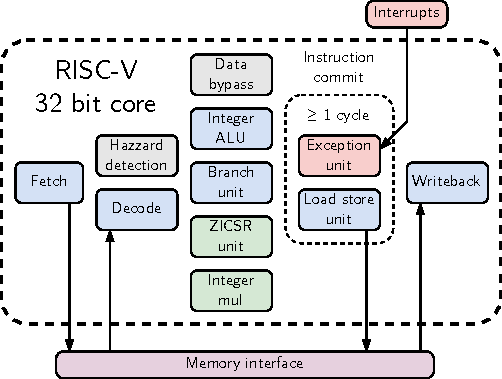
\includegraphics[width=0.8\textwidth]{root/Imagenes/3_estado_arte/riscv_core.pdf}
    \caption{Ruta de datos del procesador RISC-V utilizado. Los bloques relacionados con la arquitectura base RV32I se muestran en azul, los bloques para detectar riesgos de datos en gris, los bloques relacionados con el modo M en rojo, los bloques de extensiones estándar extra en verde y en morado el interfaz con el bus de memoria.}
    \label{fig:riscv_data_pipeline}
\end{figure}

\section{Redes Neuronales Bayesianas}

El aprendizaje automático es una rama de la inteligencia artificial que se centra en el desarrollo de algoritmos y modelos estadísticos que permiten generalizar respuestas en problemas para los que no han sido explícitamente programados aprendiendo de un conjunto de datos dado.

Las NN son modelos de aprendizaje automático cuya estructura esta inspirada en el funcionamiento de redes de neuronas biológicas \cite{deep_learning_nature}. Una NN esta compuesta por capas de neuronas conectadas entre si. Cada capa cuenta con un conjunto de pesos y una función de activación. Las NN necesitan un proceso de entrenamiento en el que son expuestas a un conjunto de datos etiquetados para que puedan ajustar el valor de los pesos de las diferentes capas. En los últimos años, las NN han obtenido muy buenos resultados en problemas de clasificación y regresión entre otros.

Las BNN son un tipo de NN que integran modelado probabilístico, lo que les permite cuantificar la incertidumbre en tareas de aprendizaje automático, mejorando su confianza y fiabilidad \cite{bnn_hyper_uncertainty}. Sin embargo, necesitan más parámetros para definir los pesos, normalmente el doble que una NN convencional, y la inferencia es más compleja. Los pesos de las BNN son distribuciones de probabilidad, normalmente distribuciones gaussianas, que se han de muestrear durante las propagaciones de la entrada. El algoritmo de inferencia más común para las BNN requiere múltiples propagaciones de la entrada de la red, aumentando drásticamente el coste computacional del mismo \cite{bnn_theory_paper}. 

La Figura \ref{fig:bnn_vs_nn_example} muestra la utilidad de las métricas de incertidumbre con un ejemplo simple. Considerando una NN convencional y una BNN ambas entrenadas para clasificar imágenes de perros y gatos, en el caso de que se les pidiera clasificar un dato anómalo, como la imagen de un tigre, con la BNN se obtendría un valor de incertidumbre alto, indicando una anomalía en la predicción, mientras que con una NN convencional no se tendría ningún indicio de que el dato de entrada era anómalo.

\begin{figure}[h]
    \centering
    \includegraphics[width=\textwidth]{root/Imagenes/3_estado_arte/nn_bnn_example.pdf}
    \caption{Ejemplo sencillo de utilidad de las métricas de incertidumbre aportadas por las BNN. Una NN convencional y una BNN, ambas entrenadas para clasificar imágenes de perros y gatos, reciben como entrada la imagen de un tigre. La BNN es capaz de detectar el dato anómalo mientras que la NN convencional no.}
    \label{fig:bnn_vs_nn_example}
\end{figure}

La Figura \ref{fig:neuron_comparation} muestra una comparación sencilla de una neurona clásica y de una neurona bayesiana, ambas con una función de activación de rectificación (\textit{\textbf{Re}ctified \textbf{L}inear \textbf{U}nit}).

% Vertically alling two sufigures and keep subcaption using floatrow and subcaptions pkgs
\begin{figure}[htb]
  \floatsetup{heightadjust=all, valign=c}
  \begin{subcaptiongroup}
  \begin{floatrow}
    \ffigbox{%
      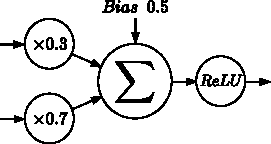
\includegraphics[width=0.48\textwidth]{root/Imagenes/3_estado_arte/clasic_neuron.pdf}
    }{%
      \caption{Neurona clásica}%
      \label{fig:clasic_neuron}%
    }
    \ffigbox{%
      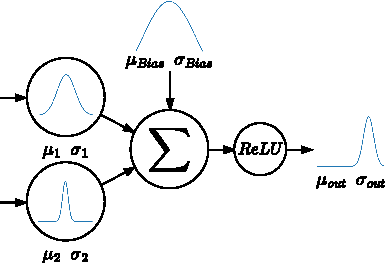
\includegraphics[width=0.49\textwidth]{root/Imagenes/3_estado_arte/bnn_neuron.pdf}
    }{%
      \caption{Neurona bayesiana}%
      \label{fig:bnn_neuron}%
    }
  \end{floatrow}
  \end{subcaptiongroup}
  \caption{Comparación de una neurona clásica con respecto a una neurona bayesiana, ambas con la misma función de activación ReLU. Los pesos de la neurona convencional son valores estáticos mientras que los de la neurona bayesiana son distribuciones gaussianas parametrizadas mediante medias y desviaciones típicas.}%
  \label{fig:neuron_comparation}%
\end{figure}

En un entorno IoT donde los datos pueden ser incompletos o ruidosos la capacidad de cuantificar la incertidumbre es crucial para tomar decisiones confiables en aplicaciones críticas. Por lo que las BNN son una muy buena herramienta para mejorar la precisión y la robustez de los sistemas de aprendizaje automático en estos entornos.

Las métricas de incertidumbre proporcionadas por las BNN son muy útiles para detectar diferentes tipos de situaciones. Por ejemplo, pueden servir para valorar la confianza de la predicción, si una predicción tiene una alta incertidumbre podría indicar que es menos confiable y que requeriría de verificación humana. También pueden utilizarse para valorar la calidad los datos de entrenamiento, si los datos de entrenamiento contienen muestras mal etiquetadas sus predicciones tendrán una mayor incertidumbre asociada. Alcolea \emph{et al.} \cite{bnn_hyper_uncertainty} \javier{ mostraron que existe una clara correlación entre la incertidumbre y la precisión en un modelo bien entrenado, por tanto la incertidumbre se puede utilizar para identificar salidas con menor probabilidad de acierto de la requerida.} También observaron que al entrenar una BNN con los datos de 2 clases mezclados se aprecia un claro incremento en la incertidumbre de las predicciones asociadas a esas clases, y que \javier{la incertidumbre aumentaba cuando se añadía ruido aleatoria a las entradas}. Otro posible uso es detectar que los datos de entrenamiento no reflejan correctamente la realidad, predicciones con alta incertidumbre pueden indicar que los datos que esta procesando el modelo no se parecen a los datos con los que ha sido entrenado. En entornos dinámicos como IoT, donde las condiciones pueden cambiar rápidamente, si la incertidumbre en las predicciones aumenta repentinamente, puede indicar un cambio en el entorno que requiera una recalibración del modelo.

\subsection{Marco teórico} \label{sec:bnn_formulas}

Estas redes neuronales utilizan el Teorema de Bayes,  ecuación \ref{eq:bayes_theo}, para modelar la probabilidad de un conjunto de pesos $w$ dado un conjunto de datos de entrenamiento $D = \{x, y\}$. Esta distribución de probabilidad es la probabilidad a posteriori.
\begin{equation} \label{eq:bayes_theo}
p(w|D) = \dfrac{p(D|w) p(w)}{p(D)}
\end{equation}

El entrenamiento de una BNN consiste en calcular esta distribución a posteriori. Calcular esta distribución para un modelo grande y complicado como una BNN es intratable. Para aproximar esta distribución se utilizan métodos inferencia bayesiana. El método más común es la inferencia variacional, que aproxima la distribución a posteriori usando una más simple $q_{\phi}(w)$. Esta aproximación se realiza minimizando la divergencia de Kullback-Leibler \cite{kl_divergence} entre $q_{\phi}(w)$ y $p(w|D)$ mediante la actualización de un conjunto de parámetros $\phi$. Teóricamente, las distribuciones podrían tener cualquier forma, pero para reducir el espacio de búsqueda solo se utilizan distribuciones simétricas y simples. Las distribuciones gaussianas son una buena opción porque solo se definen con dos parámetros, lo que ayuda a reducir el tamaño del modelo.

En consecuencia, una BNN entrenada consiste en un conjunto de medias y desviaciones de diferentes distribuciones gaussianas $\phi = \{\mu, \sigma\}$, lo que significa que los pesos se convierten en distribuciones de probabilidad en lugar de valores fijos, y la salida también se convierte en una distribución en lugar de un valor único. Esto permite medir la incertidumbre de la predicción. La Ecuación \ref{eq:bayes_inference} muestra la distribución de predicción a posteriori de una nueva observación $x^*$.
\begin{equation} \label{eq:bayes_inference}
p(y^*|x^*,D) = \int p(y|x^*,w) p(w|D) dw
\end{equation}

Mediante métodos de Monte Carlo se puede aproximar la integral de la Ecuación \ref{eq:bayes_inference}. En este caso, las muestras son diferentes propagaciones estocásticas de la entrada. En cada una de estas propagaciones, los pesos se muestrean de las distribuciones gaussianas que forman la distribución a posteriori aproximada.

Siendo $T$ el número de muestras, $K$ el número de clases posibles y una muestra $a_t$ el vector de longitud $K$ de componentes $p(y^* = c_k | x^*, w_t)$. Cada uno de sus componentes representa la probabilidad de que $y^*$ sea $c_k$. Para obtener una única predicción se puede tomar el componente máximo del vector promedio de todas las muestras.

\subsubsection{Cálculo de la incertidumbre}

En problemas de clasificación, se puede medir la incertidumbre de una predicción utilizando las diferentes muestras Monte Carlo obtenidas \cite{uncertainty_metrics}. A continuación se explica como obtener las métricas mas relevantes y lo que representan.

La incertidumbre predictiva ($\mathbb{H}$) representa la incertidumbre de una predicción en el rango $[0, \log(K)]$ y puede calcularse utilizando la Ecuación \ref{eq:predictive_uncertainty}.
\begin{equation} \label{eq:predictive_uncertainty}
\mathbb{H}(y|x,D) = - \sum^K_{k=1} \left[ \left( \dfrac{1}{T} \sum^T_{t=1} a_t \right) \log\left( \dfrac{1}{T} \sum^T_{t=1} a_t \right) \right]
\end{equation}

La incertidumbre puede dividirse en dos, aleatoria y epistémica, $\mathbb{H}$ captura ambas. La entropía esperada ($\mathbb{E}p$) captura la incertidumbre aleatoria, que es causada por ambigüedades en el conjunto de datos como mediciones ruidosas, clases superpuestas o muestras mal etiquetadas. $\mathbb{E}p$ puede calcularse utilizando la Ecuación \ref{eq:expected_entropy}.
\begin{equation} \label{eq:expected_entropy}
\mathbb{E}{p(w|D)}[\mathbb{H}(y|x,D)] = \dfrac{1}{T} \sum^T{t=1} \left( -\sum^K_{k=1} a_{t} \log(a_t) \right)
\end{equation}

La incertidumbre epistémica representa lo que el modelo no sabe debido a la falta de datos durante el proceso de entrenamiento, y puede calcularse utilizando la información mutua (\textit{\textbf{M}utual \textbf{I}nformation}) mostrada en la Ecuación \ref{eq:mutual_information}.
\begin{equation} \label{eq:mutual_information}
MI(y,w|x,D) = \mathbb{H}(y|x,D) - \mathbb{E}_{p(w|D)}[\mathbb{H}(y|x,D)]
\end{equation}

\subsection{Aceleración hardware}

La aceleración de algoritmos de aprendizaje automático es un campo de investigación muy activo con muchas propuestas recientes \cite{survey_ai22}. La aceleración de las BNN no es una excepción, debido en parte al elevado coste de su algoritmo de inferencia. Otros trabajos se han centrado en desarrollar aceleradores de alto rendimiento para el proceso completo de inferencia \cite{bnn_grng_accel, sampling_free_bnn_accel, bnn_clt_approx}.

Awano \emph{et al.} propusieron un acelerador sin múltiples propagaciones ni muestreo para el algoritmo de inferencia de las BNN, reemplazando la función de activación ReLU por una función cuadrática \cite{sampling_free_bnn_accel}. Su trabajo muestra buenos resultados para el conjunto de datos MNIST, pero otros trabajos han demostrado que este enfoque no es generalizable y no funciona bien con otros modelos \cite{bnn_clt_approx}. Por esta razón, este trabajo se centra en el algoritmo de múltiples propagaciones con muestreo, ya que es el método más estándar y ha sido ampliamente demostrado que da buenos resultados para varios diferentes conjuntos de datos \cite{bnn_grng_accel, bnn_clt_approx, bnn_hyper_uncertainty}.

El muestreo de distribuciones para generar los pesos es una parte fundamental de los trabajos que siguen el enfoque de múltiples propagaciones. Cai \emph{et al.} propusieron un acelerador de inferencia de BNN con 2 posibles GRNG \cite{bnn_grng_accel}. Uno basado en el teorema central del límite (TCL) utilizando la distribución binomial y otro en el método de Wallace \cite{wallace_grng}.

Los GRNG son un tema que ya ha sido explorado en profundidad \cite{grng_survey}. Trabajos anteriores han mostrado que los GRNG basados en el CLT no muestran una precisión elevada en la cola de la distribución \cite{clt_grng}. Sin embargo, en el caso de la inferencia de las BNN no es necesario tener un GNRG preciso. Hirayama \emph{et al.} demostraron que utilizando un GRNG de poca precisión basado en una \textit{Lookup Table} (LUT) se obtienen buenos resultados \cite{bnn_lut_grng}.

En otro trabajo Awano \emph{et al.} diseñaron un acelerador que aproximan la salida final del modelo utilizando generadores hardware de muestras Bernoulli \cite{bnn_clt_approx}, bajo la condición de que el TCL podría aplicarse al modelo en general. La Figura \ref{fig:b2n2_clt} muestra un diagrama de su aproximación.

\begin{figure}[h]
    \centering
    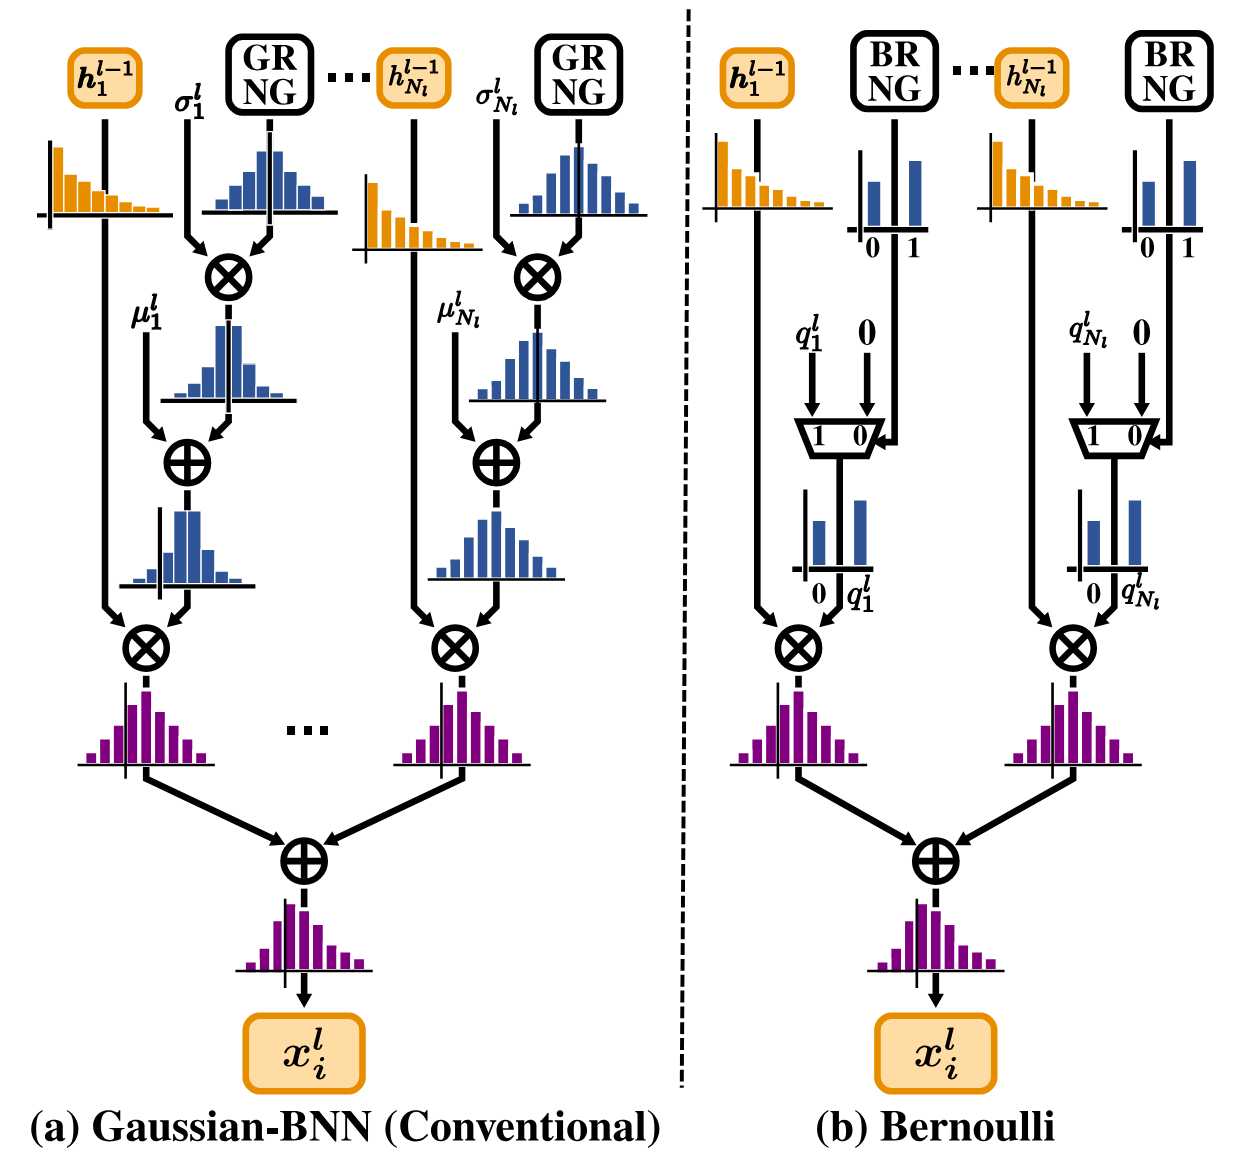
\includegraphics[width=0.55\textwidth]{root/Imagenes/3_estado_arte/b2n2_clt.png}
    \caption{Comparación de muestrear distribuciones gaussianas o distribuciones de Bernoulli en una BNN. Debido al TCL la distribución final es independiente de las distribuciones muestreadas \cite{bnn_clt_approx}.}
    \label{fig:b2n2_clt}
\end{figure}

Una ventaja clave de los generadores de muestras Bernoulli radica en su implementación en hardware. A diferencia de los métodos de software que dependen de operaciones de salto, que pueden degradar el rendimiento de las CPU modernas, los generadores hardware pueden implementarse utilizando componentes simples como comparadores y multiplexores, lo que los hace de bajo coste y eficientes.

\subsection{Soporte de bibliotecas}

Este trabajo tiene como objetivo ejecutar inferencia de estas redes en entornos RISC-V de bajas prestaciones, donde actualmente no existe un conjunto de bibliotecas que lo permita. TensorFlow Probability permite entrenar y ejecutar inferencia de BNN utilizando precisión en punto flotante. Por otro lado, en el caso de PyTorch, existe BayesianTorch desarrollado por IntelLabs \cite{bayesian_torch}, que ofrece la misma funcionalidad.

TensorFlowLite \cite{tflite} es la versión de TensorFlow diseñada para sistemas empotrados, ofrece funcionalidades como la cuantización de modelos y la inferencia utilizando precisión de enteros para las NN convencionales. Sin embargo, aun no soporta BNN. En una actualización reciente, BayesianTorch ha añadido soporte para la cuantización de BNN \cite{bnn_quant}. Este trabajo se centra en el ecosistema de Tensorflow debido a que se han utilizado modelos desarrollados dicho entorno para su validación. 
